\lohead{Florian Greistorfer}
\chapter{Webserver und Client}

\section{Begriffserklärungen}

\subsection{Server}
Ein Computer oder Programm, der oder das Zugriff auf eine Resource oder einen Dienst in einem Netzwerk ermöglicht

\subsection{Client}
Ein Computer oder Programm, der oder das auf einen Server Zugreift

\section{Anforderungen}

\subsection{Webserver}
Auf der Katzenfütterungsanlage läuft ein Webserver, der es ermöglicht, dass der Benutzer das Gerät über das Internet erreichen kann. Hauptaufgaben des Servers sind dabei, Daten bereitzustellen, zu verabeiten und zu speichern und den Webclient zur Verfügung zu stellen.

\subsection{Client}
Der Client soll dem Benutzer ermöglichen, die Katzenfütterungsanlage über einen Webbrowser zu steuern. Ein Benutzername und ein Passwort sind erforderlich, damit man das Gerät bedienen kann. Das Design soll eindeutig und übersichtlich gehalten sein. Auf der Startseite sollen die eingestellten Fütterungszeiten zu sehen sein und eine allgemeine Übersicht. Über eine Navigationsleiste sollen die weiteren Seiten erreichbar sein:

\begin{itemize}
\item[•]Fütterrungszeiten
\item[•]Positionsinfo
\item[•]Geräteinfo
\item[•]Update
\end{itemize}



\section{Voruntersuchung}

\subsection{Typescript}
Typescript ist eine Weiterentwicklung der Sprache Javascript, die strenge Datentypen hat. Typescript muss von einem Transpiler (=Übersetzer) in Javascript übersetzt werden. Javascript kann direkt von jedem herkömmlichen Browser ausgeführt werden.
\subsection{Node.js}
Node.js ist eine Laufzeitumgebung, die es ermöglicht, dass Javascript direkt auf einem Rechner ausgeführt werden kann. 

\subsection{Angular 2/4}
Angular ist ein Typescript Framework, das aus dem Javascript-Framework AngularJS weiterentwickelt wurde. Es wird von Google entwickelt. Angular ist gegliedert in Komponenten. Die grobe Struktur wird in der Abbildung \ref{Angular Struktur} dargestellt.

\begin{figure}[H]
      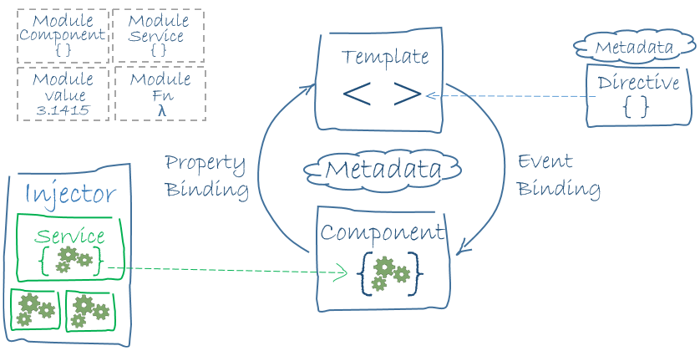
\includegraphics[width=1\textwidth]{Bilder/Greistorfer/Angular.png}
      \caption{Angular Struktur}
      \label{Angular Struktur}
\end{figure}

\subsubsection{Modules}

\subsubsection{Components}

\subsubsection{Templates}

\subsubsection{Data binding}

\subsubsection{Services}

\subsection{Bootstrap}
Bootstrap 

\section{Umsetzung}

\subsection{Client}

\subsubsection{Design}
Das Design sollte übersichtlich und einfach gestaltet werden. Der Benutzer soll auf den ersten Blick die wichtigsten Funktionen und Informationen erkennen können. \\

\begin{wrapfigure}{r}{0.7\textwidth}
\vspace{-30pt}
  \begin{center}
    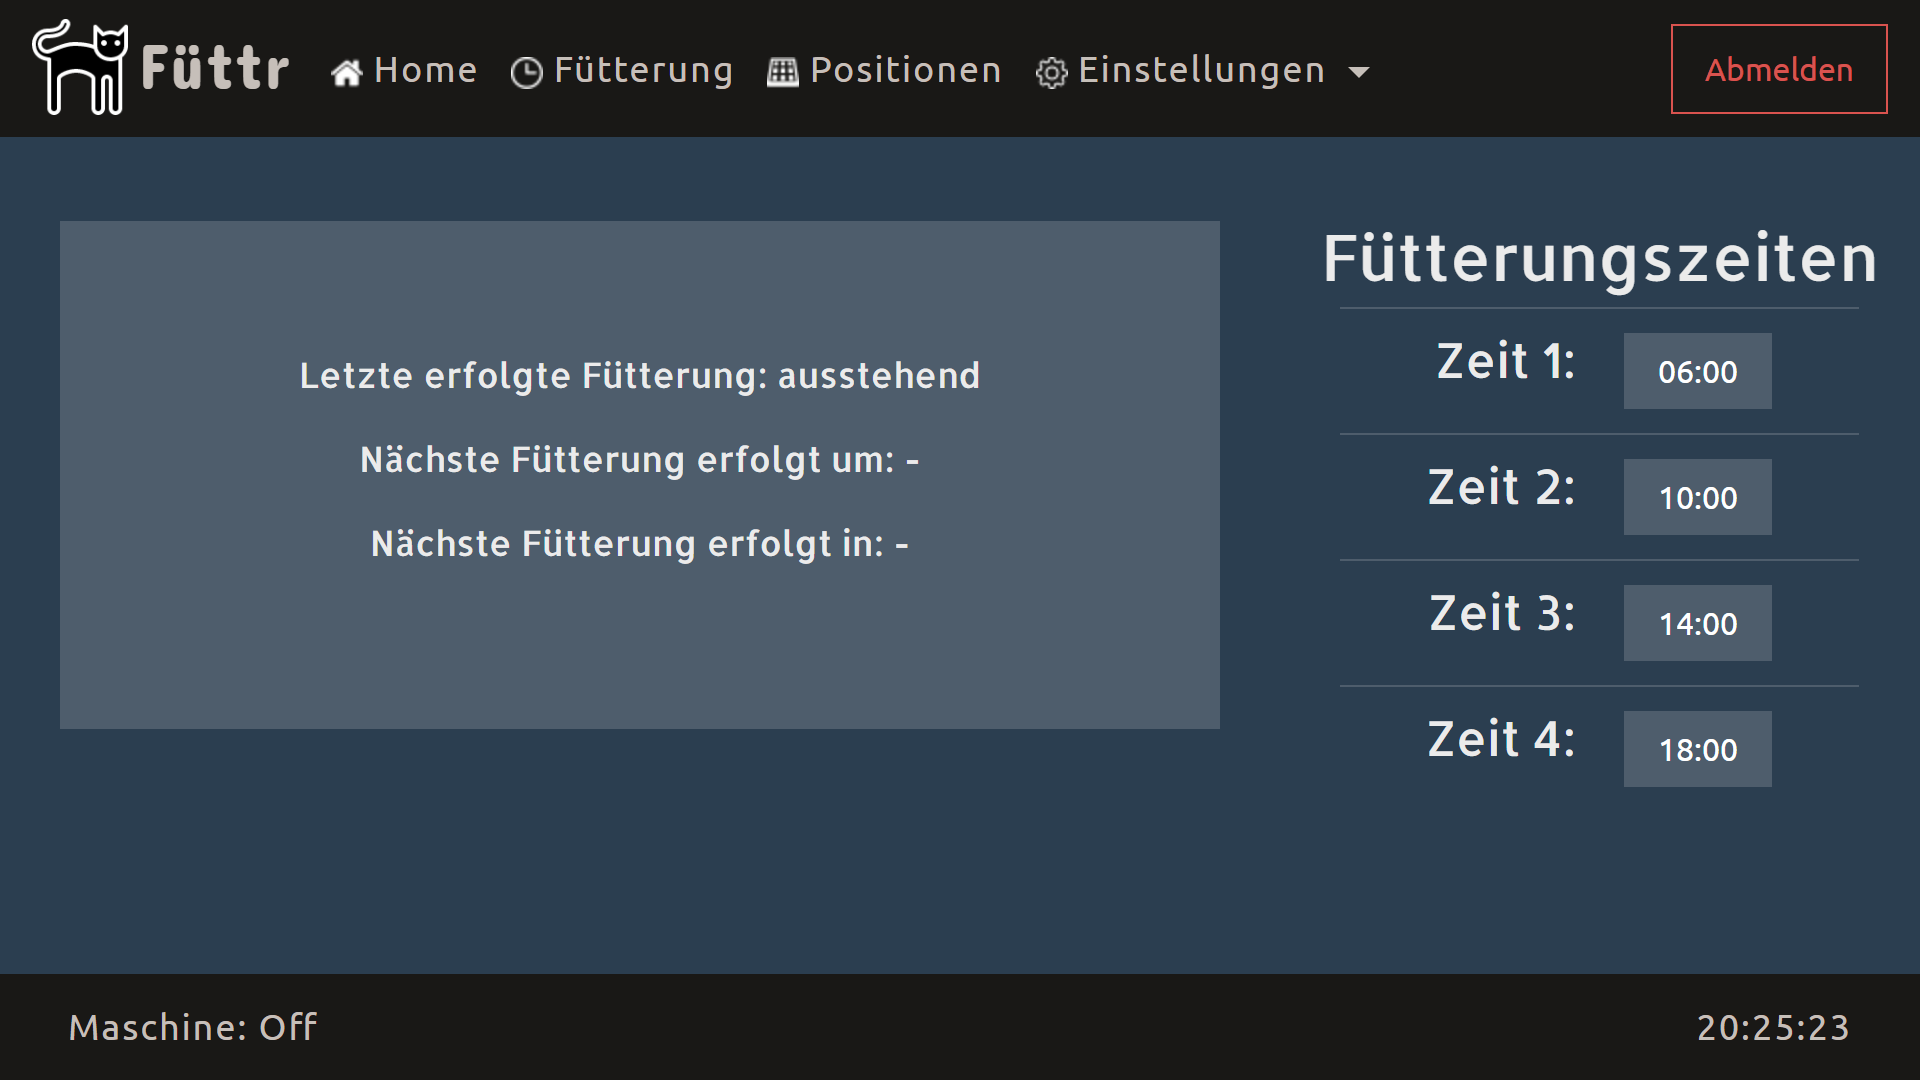
\includegraphics[width=0.7\textwidth]{Bilder/Greistorfer/Home.png}
  \end{center}
  \caption{Startseite}
  \label{Startseite}
  \vspace{-10pt}
\end{wrapfigure}

Auf der Starseite sind alle wichtigen Informationen übersichtlich dargestellt. Auf der linken Seite werden die Uhrzeit der letzten erfolgreichen Fütterung, die Zeit der nächsten Fütterung und die Zeit bis zur nächsten Fütterung dargestellt. Darunter werden Fehler und Warnungen, fals welche auftreten sollten, angezeigt. Da unbekannt ist, wie viele Fehler und Warnungen auftreten, werden diese in einem *ngFor aufgelistet. Auf der rechten Seite sind die aktiven Fütterungszeiten aufgelistet.

\begin{lstlisting}[style=HtmlStyle,caption=Errors and Warnings in einem *ngFor]
<ul style="list-style-type: none; margin-left: -40px;">
	<li *ngFor="let warning_message of ErrorsAndWarnings.Warnings">
    	<div class="alert alert-warning alert-dismissable fade show" [hidden]="warning_message.hidden">
        	<button type="button" class="close">
            	<span aria-hidden="true" (click)="ack(warning_message)">&times;</span>
            </button>
            <strong i18n>Warning! </strong>{{warning_message.message}}
        </div>
    </li>
    <li *ngFor="let error_message of ErrorsAndWarnings.Errors">
        <div class="alert alert-danger alert-dismissable fade show" [hidden]="error_message.hidden">
	        <button type="button" class="close">
	            <span aria-hidden="true" (click)="ack(error_message)">&times;</span>
            </button>
            <strong i18n>Error! </strong>{{error_message.message}}
        </div>
    </li>
</ul>
\end{lstlisting}

\begin{wrapfigure}{r}{0.7\textwidth}
\vspace{-30pt}
  \begin{center}
    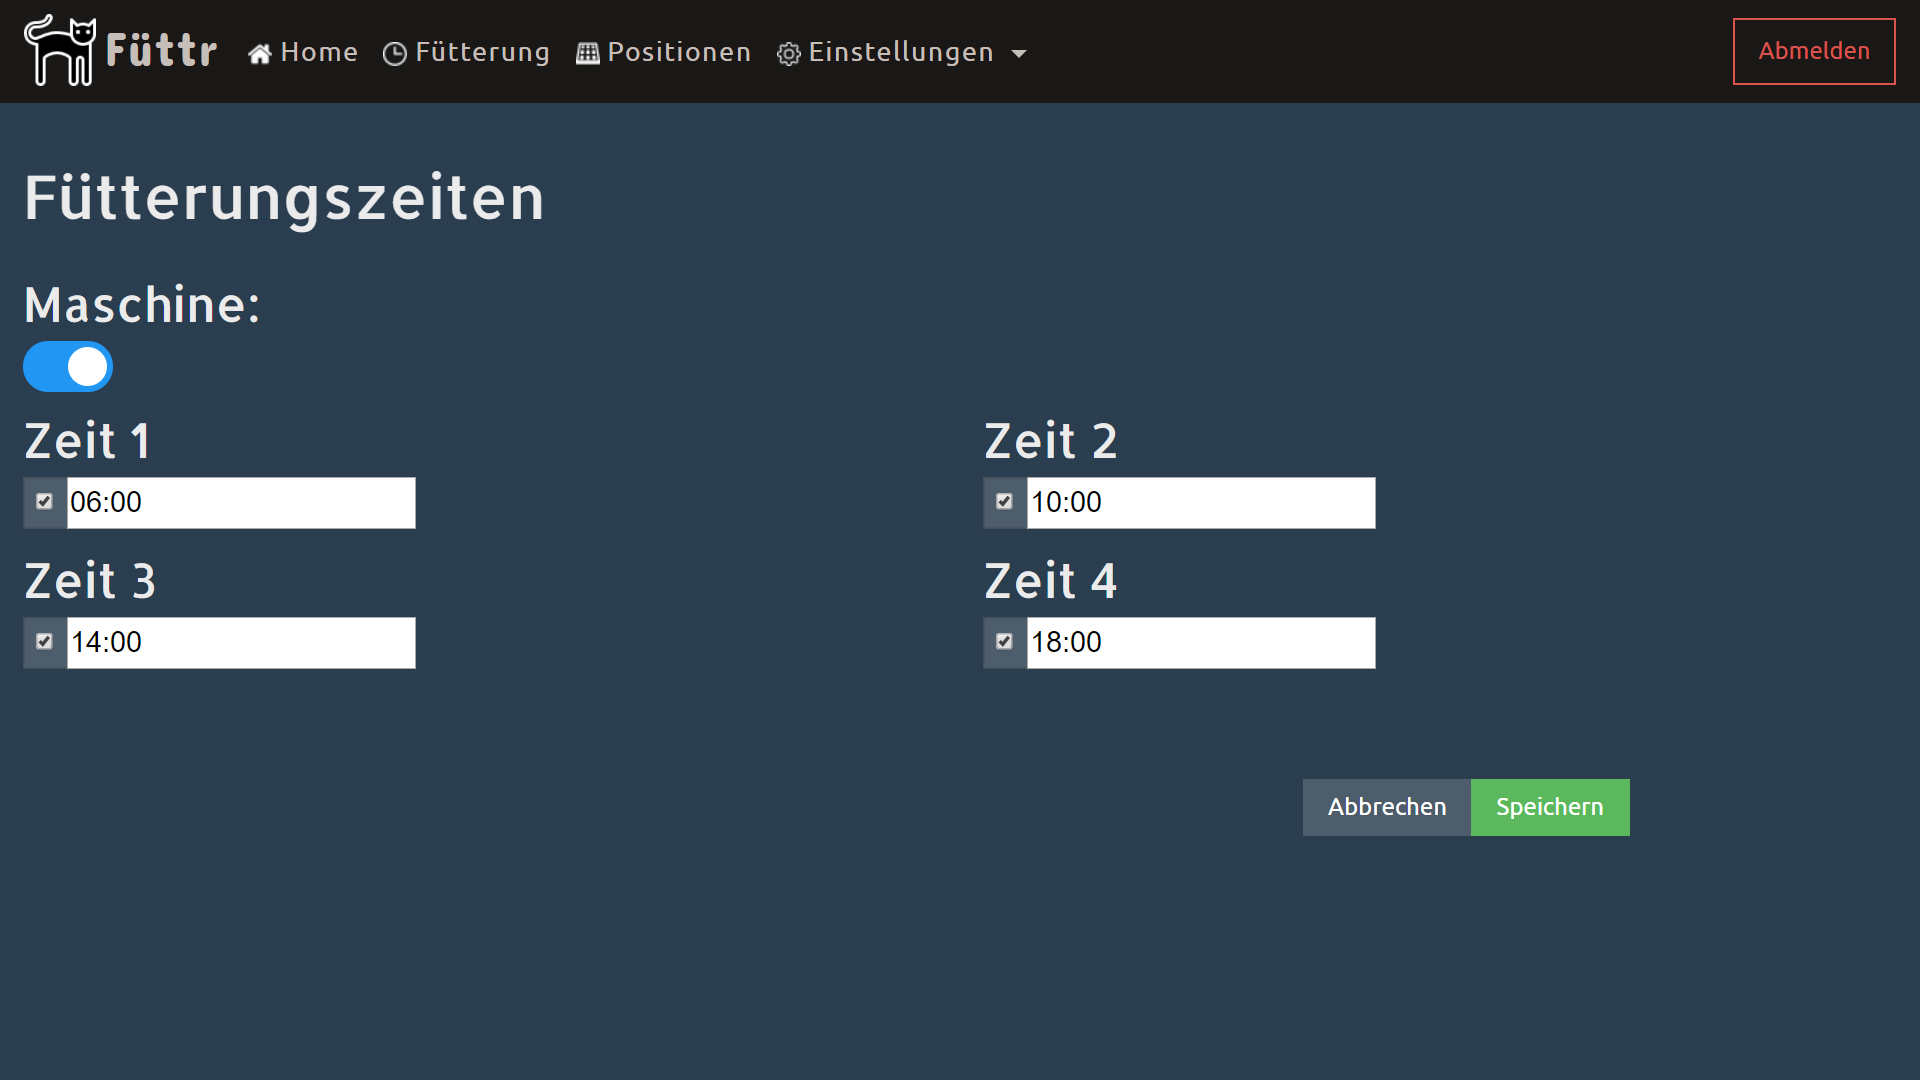
\includegraphics[width=0.7\textwidth]{Bilder/Greistorfer/Fuetterungszeiten.png}
  \end{center}
  \caption{Fütterungszeiten}
  \label{Fütterungszeiten}
  \vspace{-10pt}
\end{wrapfigure}

Auf der Fütterungszeiten-Seite kann der Benutzer die Katzenfütterungsanlage ein und ausschalten, außerdem

\begin{wrapfigure}{r}{0.7\textwidth}
\vspace{-30pt}
  \begin{center}
    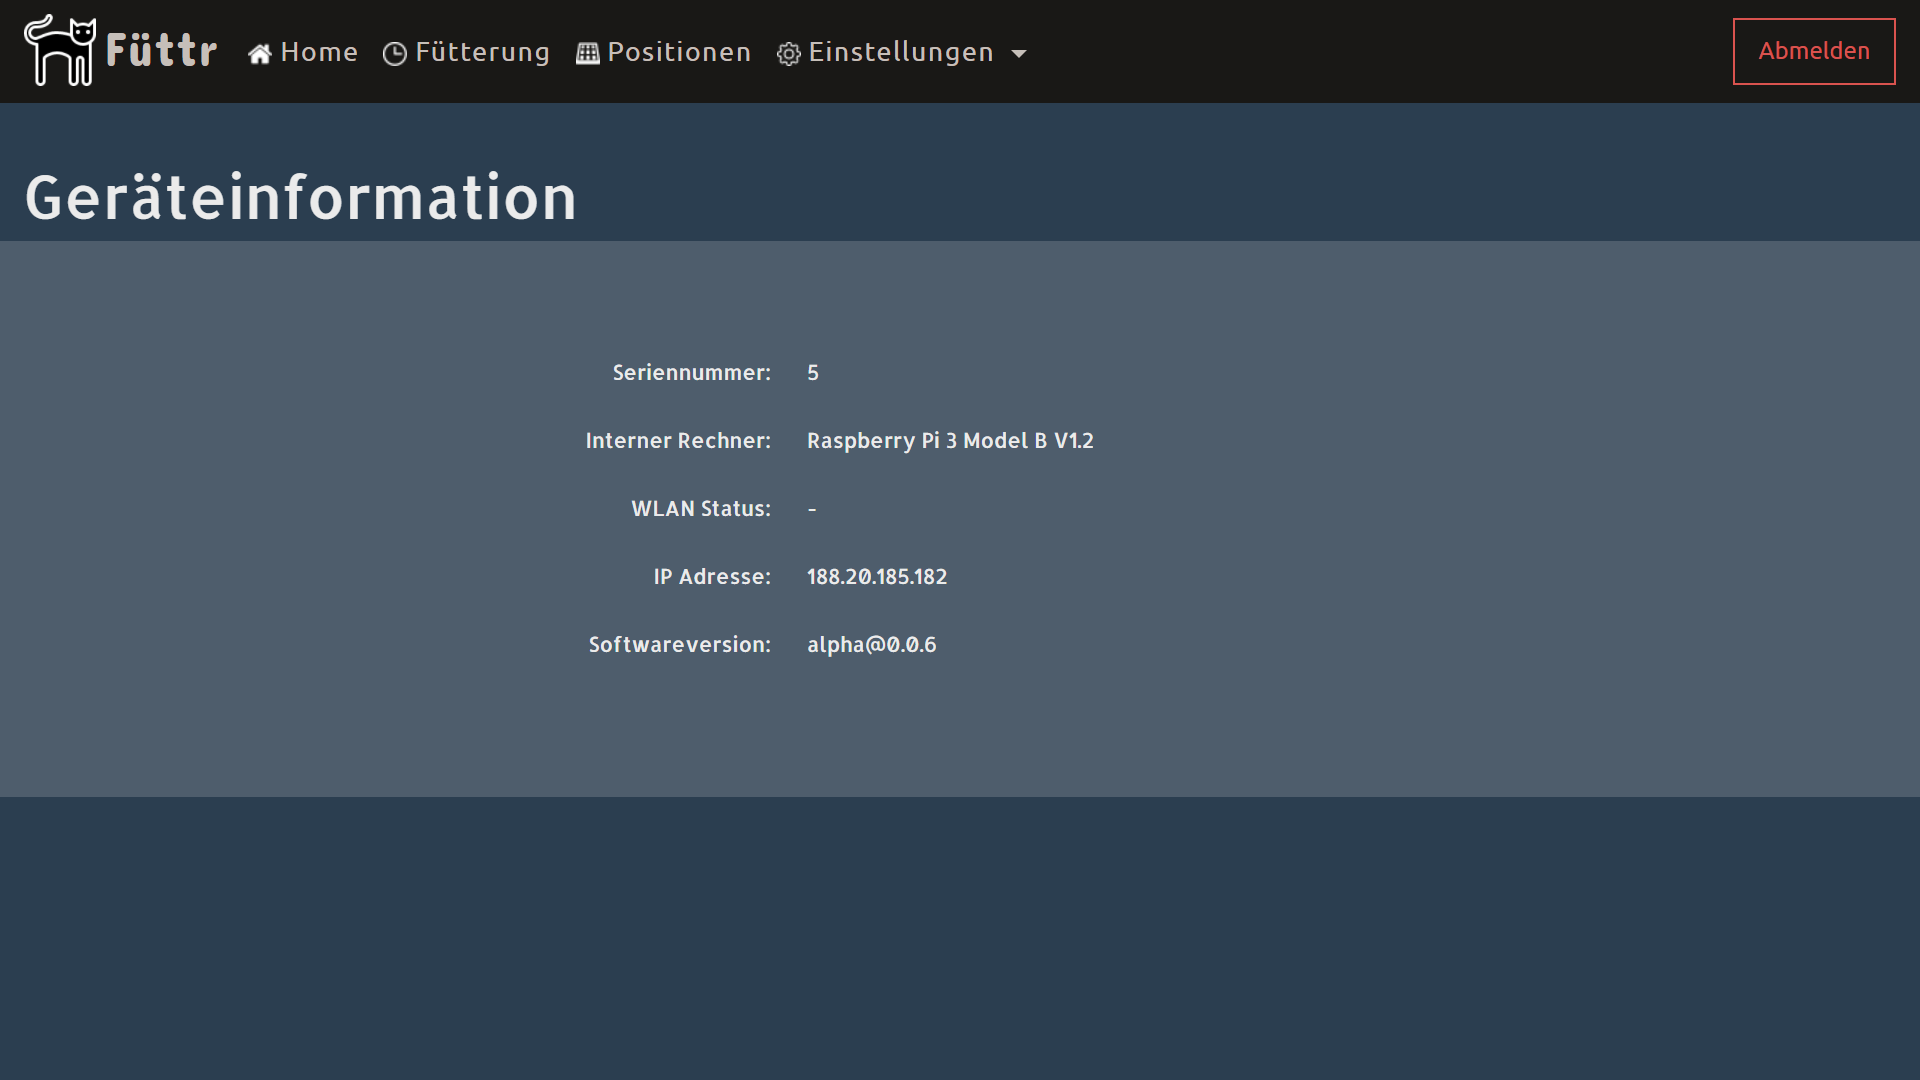
\includegraphics[width=0.7\textwidth]{Bilder/Greistorfer/Gerateinformation.png}
  \end{center}
  \caption{Geräteinformationen}
  \label{Geräteinformationen}
  \vspace{-10pt}
\end{wrapfigure}

\begin{wrapfigure}{r}{0.7\textwidth}
\vspace{-30pt}
  \begin{center}
    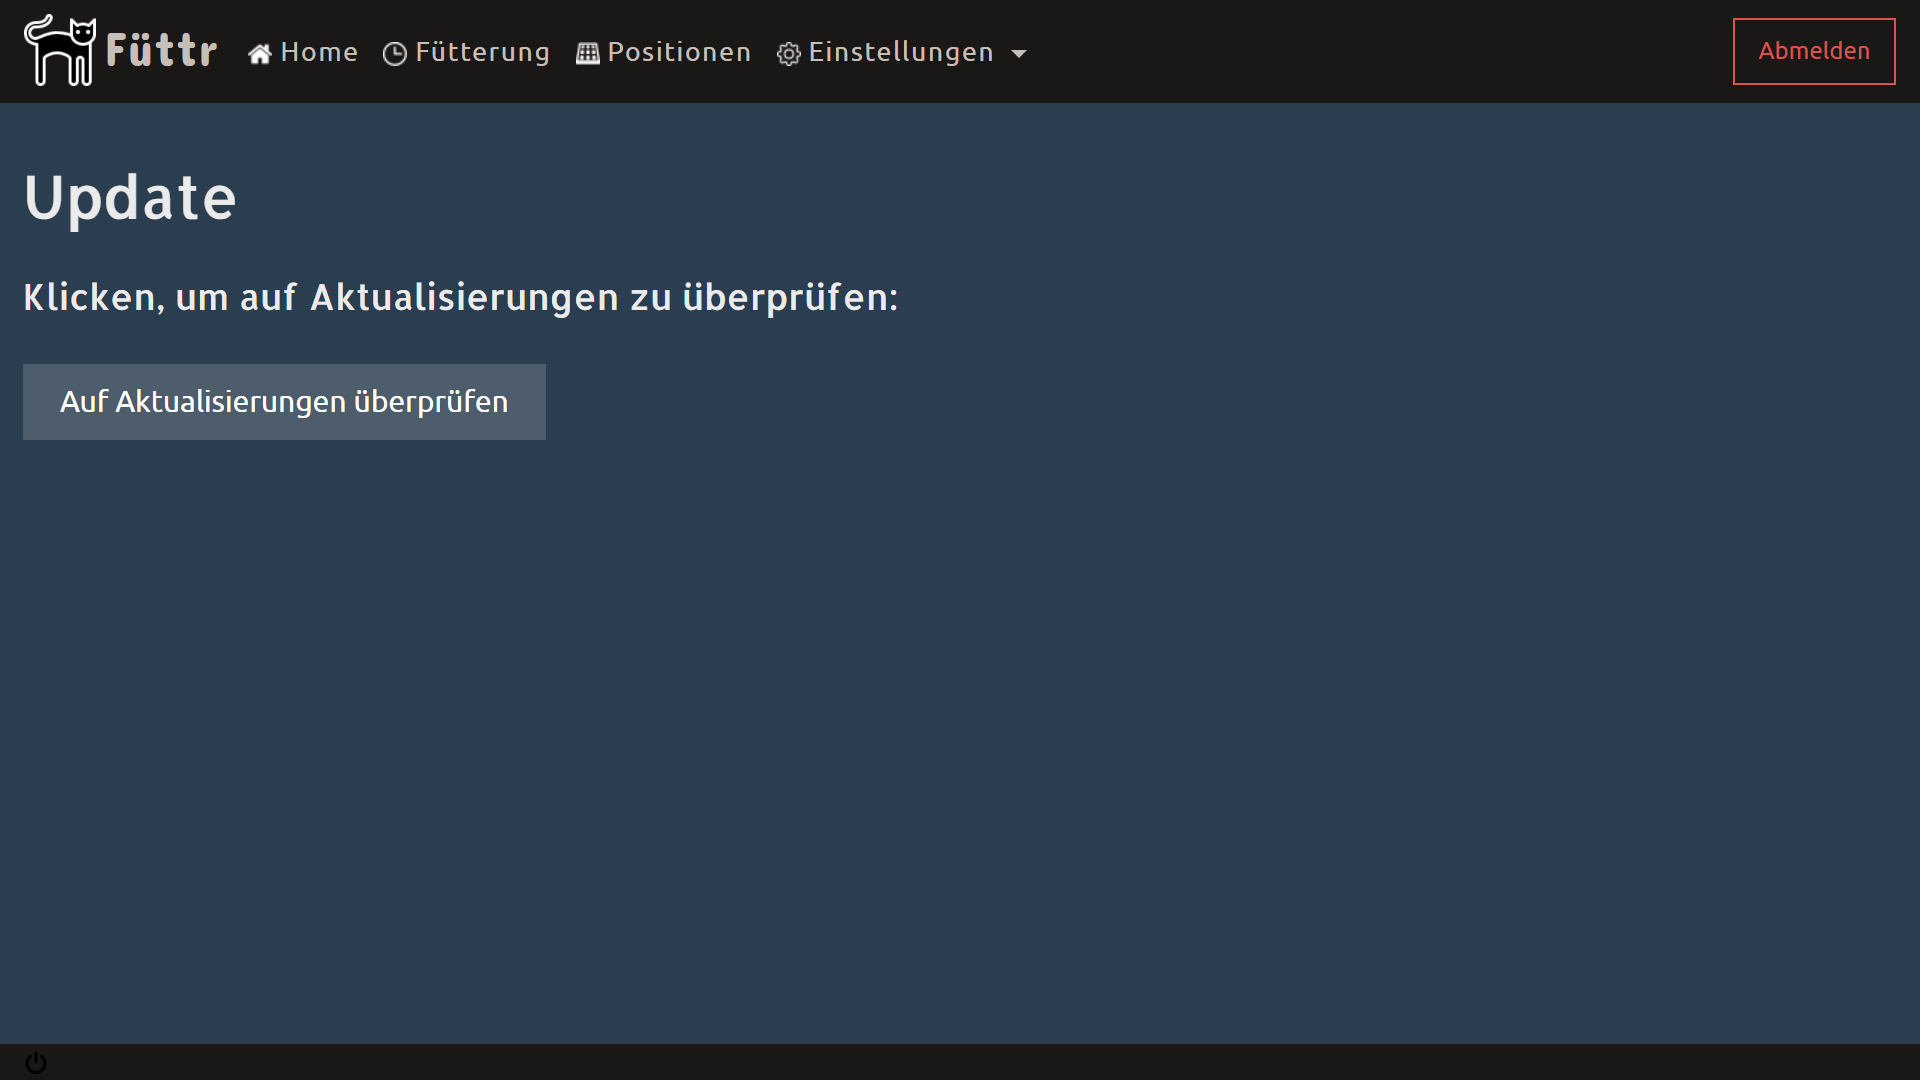
\includegraphics[width=0.7\textwidth]{Bilder/Greistorfer/Update.png}
  \end{center}
  \caption{Update}
  \label{Update}
  \vspace{-10pt}
\end{wrapfigure}

\subsubsection{Funktion}

\subsection{Server}

\subsubsection{Funktion}

\subsubsection{Mongodb}

\subsubsection{Kommunikation mit dem Java Programm}

\section{Zusammenfassung und Verbesserungsmöglichkeiten}